Per la  dimostrazione pratica degli argomenti fino a quì presentati si è scelto di progettare e implementare un applicativo software per dispositivi mobili.

L'analisi della gamma di dispositivi utilizzabili e reperibili dal team di questo progetto ha evidenziato due architetture su cui sviluppare l'applicativo: IOS e Android.

Entrambe le architetture sono parimente valide ai fini del progetto ma dovendosi confrontare con il tempo a disposizione e le conoscenze già in possesso dagli elementi del gruppo di sviluppo si è deciso di convogliare interamente le energie sullo sviluppo su piattaforma Android.

Le motivazioni di tale scelta sono le seguenti:

\begin{enumerate}
    \item La rete neurale è stata sviluppata in Tensorflow (vedi \ref{cha:reteneurale}) che ha nativamente grande interoperabilità con l'ambiente Android.
    \item Parte del gruppo di lavoro ha esperienza con lo sviluppo di applicazioni in Android nativo.
\end{enumerate}

Tutti i file e le risorse progettate e realizzate per questo progetto sono reperibili nel seguente repository \textit{GitHub}:

\begin{center}
    \url{https://github.com/DaniDF/eye_pupil_tracker}
\end{center}

\section{Schermate}
\label{sec:schermate}
L'applicazione per dimostrare l'utilizzo e il funzionamento della rete neurale implementa 3 sezioni:

\begin{itemize}
    \item \textbf{"\textit{Nerd}"} (vedi \ref{sec:nerdmde}) dove vengono mostrate tutte le informazioni che è in grado di acquisire il dispositivo e che la rete neurale processa.
    
    \item \textbf{\textit{Calibration}} (vedi \ref{sec:calibration}) schermata in cui vengono mostrate elementi grafici in modo da capire il range di movimento degli occhi nello spazio.
    
    \item \textbf{\textit{Game}} (vedi \ref{sec:game}) viene implementato un semplice gioco che sfrutti il movimento degli occhi per eseguire comandi e azioni che facciano evolvere l'utente nel gioco.
\end{itemize}

\section{Nerd Mode}
\label{sec:nerdmde}
\begin{figure}[htbp]
    \centering
    \subfigure[Schermata Nerd layout]{
    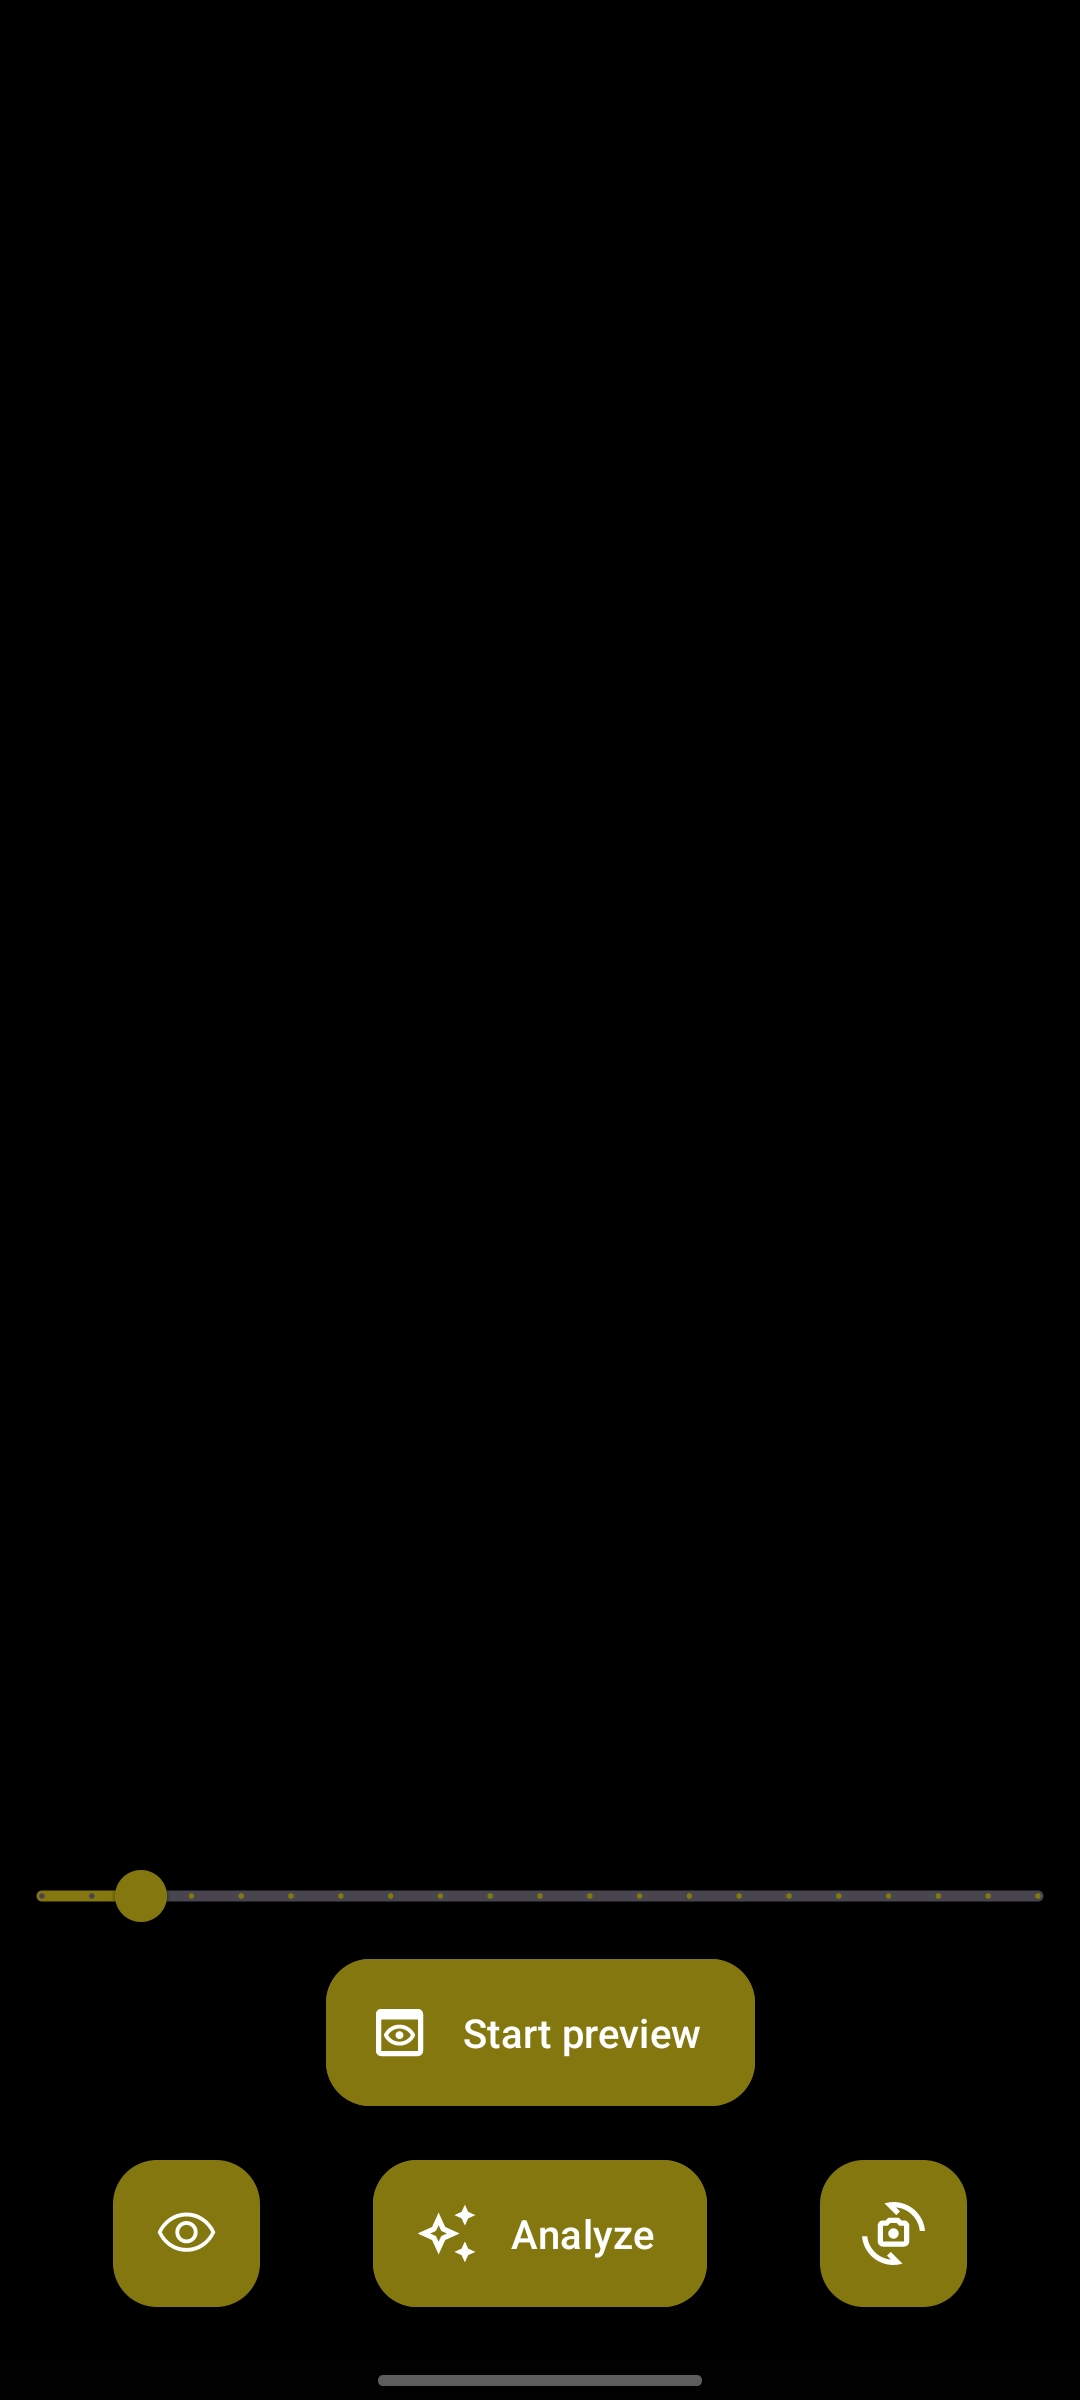
\includegraphics[scale=0.13]{ProgettoAndroid/NerdMode/Images/CameraApp_Screen_nerd_layout.jpg}
    \label{fig:nerdmodelayout}
    }
    \subfigure[Schermata Nerd mode con camera attiva]{
    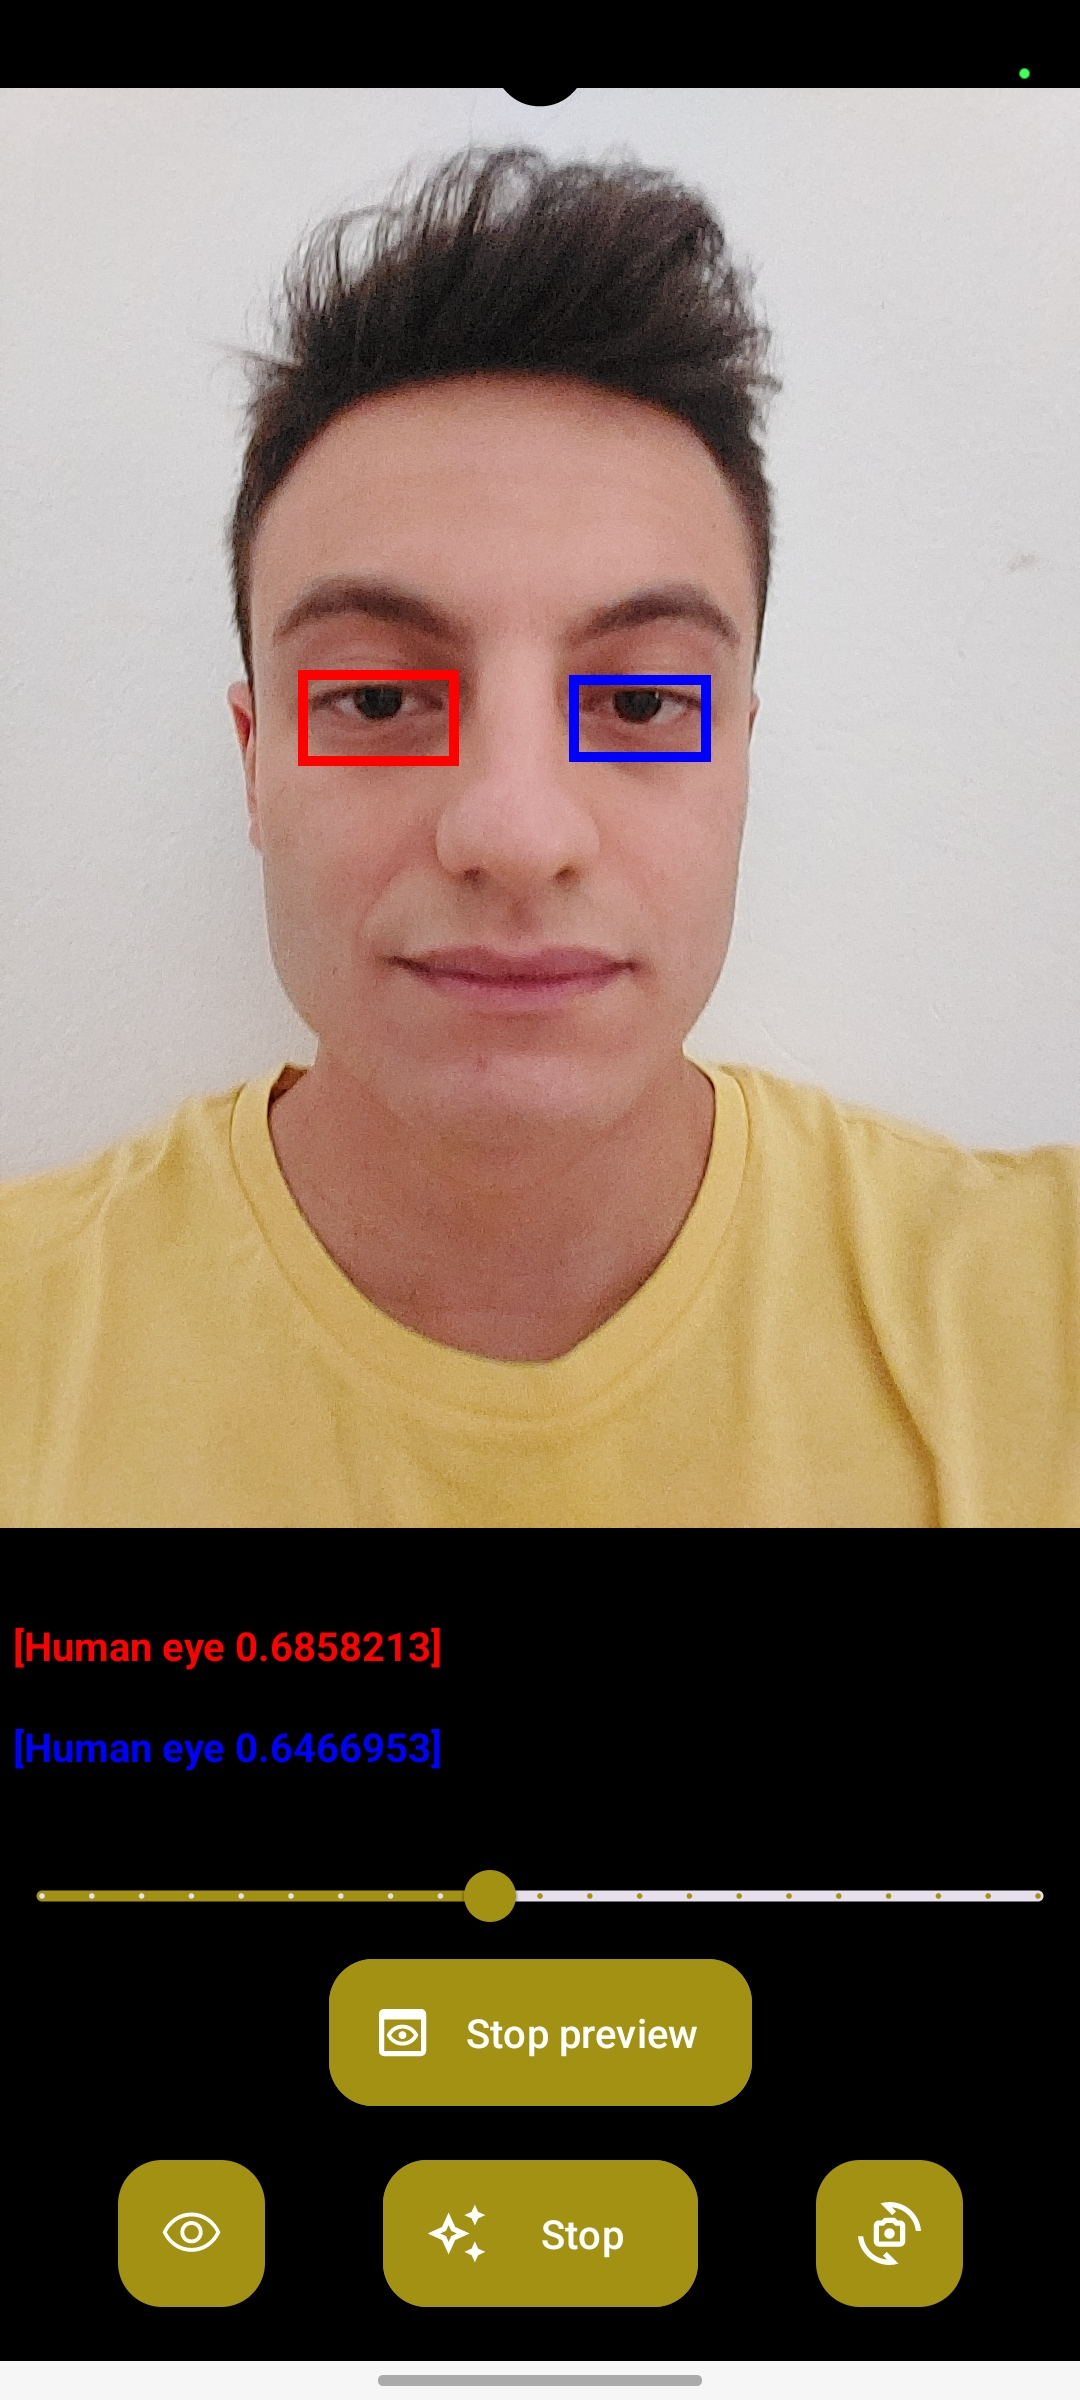
\includegraphics[scale=0.13]{ProgettoAndroid/NerdMode/Images/CameraApp_Screen_nerd.jpg}
    \label{fig:nerdmode}
    }
    \caption{Schermata Nerd}
    \label{fig:nerd}
\end{figure}

La schermata "\textit{Nerd}" è stata pensata per mostrare in modo grafico e con la maggior facilità possibile tutte le informazioni che la telecamera del dispositivo è in grado di acquisire.

Nella parte più alta dello schermo viene mostrato ciò che la telecamera acquisisce e sovrapposto l'analisi della stessa immagine tramite la rete neurale.

Per ogni occhio rilevato dalla rete neurale appare a schermo un rettangolo di colori diversi per evidenziare in che posizione è stata effettuato il tracciamento. Ulteriormente viene indicato per ogni identificazione qual è la sua accuratezza con un valore numerico decimale nell'intervallo $[0,1]$.

\subsection{Preview}
\label{sub:preview}
Il bottone "\textit{Start preview}" (vedi figura \ref{fig:nerdmodelayout}) avvia l'acquisizione dalla fotocamera del dispositivo, come fotocamera predefinita viene utilizzata quella "interna" ovvero quella rivolta verso l'utente. È possibile anche usare la fotocamera "esterna" mediante il bottone "\textit{Switch Camera}" (vedi \ref{sub:switchcamera}).

La dimensione della \textit{preview view} deve essere adattata alla dimensione del sensore della camera e quindi dell'immagine risultante. Queste dimensioni dipendono sia dal dispositivo su cui viene eseguita l'applicazione sia da quale fotocamera viene selezionata, pertanto dinamicamente l'applicazione deve adattare le dimensioni della \textit{preview view} e coerentemente il layer su cui vengono disegnati i rettangoli di tracking degli occhi. Se questa operazione non venisse effettuata o non eseguita dinamicamente la rete opererebbe comunque in maniera corretta ma la visualizzazione dei risultati risulterebbe completamente errata mostrando l'occhio in in punto dello schermo e il corrispondente rettangolo in una posizione diversa.

\subsection{Switch camera}
\label{sub:switchcamera}
Il bottone "\textit{Switch camera}" (vedi figura \ref{fig:nerdmodelayout}) permette di scegliere quale camera utilizzare per la visualizzazione e per la successiva analisi. La scelta è tra la fotocamera "interna" ovvero quella rivolta verso l'utente, lato schermo, e quella "esterna" nell'altro lato del dispositivo.

Per l'acquisizione dalla camera viene utilizzato in framework \textbf{CameraX}\cite{camerax_overview} e per costruzione, nell'attuale stato dell'arte, non permettere di scegliere, se disponibili, quale delle fotocamere esterne utilizzare, verrà dunque utilizzata in modo automatico la fotocamera esterna principale.

\subsection{Analyze}
\label{sub:analyze}
Il bottone "\textit{Analyze}" (vedi figura \ref{fig:nerdmodelayout}) è abilitato ad essere premuto sono quando è contemporaneamente abilitata la funzione "\textit{Preview}".

Alla pressione del bottone viene innescata l'analisi in tempo reale delle immagini acquisite e passate alla rete neurale per il processamento \textit{Eye-Tracking} (vedi \ref{sec:eyedetection}).

Al termine dell'analisi i risultati del tracciamento vengono mostrati a schermo su un livello grafico sovrapposto a quello di \textit{preview} della camera. Si ottiene una visualizzazione del contorno degli occhi trovati tramite rettangolo colorato e la corrispettiva accuratezza (vedi \ref{fig:nerdmode}).

È stato fondamentale gestire correttamente l'orientamento dell'immagine qualora l'utente cambi fotocamera. La fotocamera interna infatti produrrà un risultato specchiato rispetto alla visualizzazione, pertanto prima di mostrare a video i risultati ottenuti andranno orientati in base alla camera d'origine di tali dati.

Posizionato immediatamente sotto la parte di \textit{preview} è stato aggiunto uno \textit{slider} che permette di filtrare i risultati ottenuti tramite valore minimo di accuratezza.

\subsection{Attività progettuale: Riconoscimento pupilla}
\label{sub:riconoscimentopupilla}
Il bottone "\textit{Pupil-Tracking}" (vedi figura \ref{fig:nerdmodelayout}) è abilitato solo qualora sia già in esecuzione l'analisi dell'immagine.

La funzionalità di "\textit{Pupil-Tracking}" acquisisce per ogni occhio rilevato dalla fase di analisi dell'immagine un occhio e su questa porzione di immagine avvia il rilevamento della pupilla.

Al termine del processamento della rete per il riconoscimento della pupilla (vedi \ref{sec:gazedetection}) i risultati vengono mostrati a video nelle stesse modalità di quelle descritte per "\textit{Eye-Tracking}".

Qui di seguito un test effettuato direttamente su Android Studio:

\begin{figure}[htbp]
    \centering
    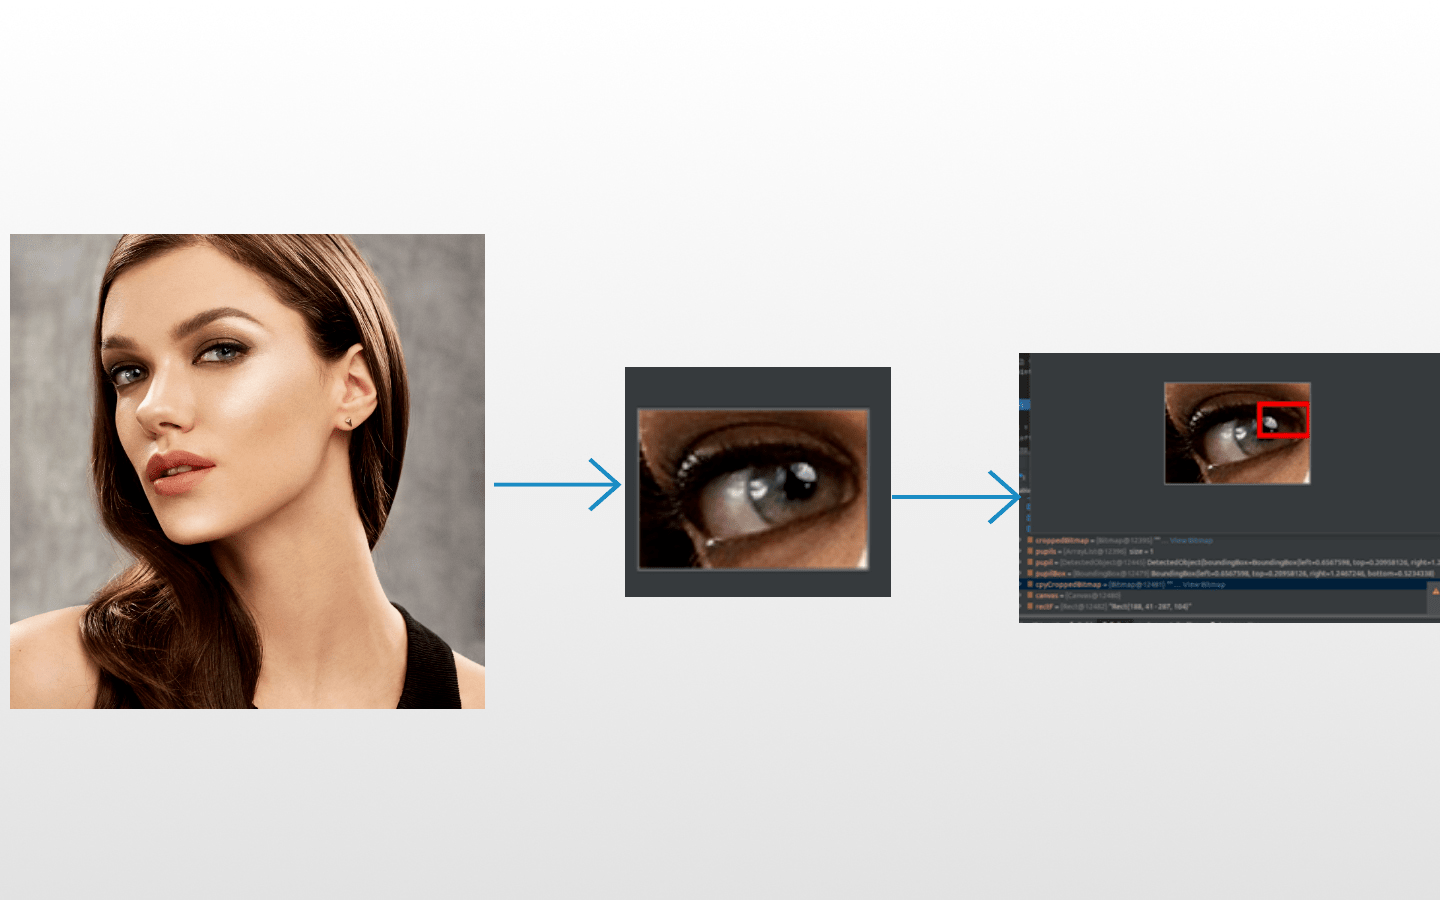
\includegraphics[scale=0.24]{ProgettoAndroid/NerdMode/RiconoscimentoPupilla/Images/gazeAndroid.png}
    \caption{Schermata Nerd mode con pupilla}
    \label{fig:nerdmodepupil}
\end{figure}

\section{Calibration}
\label{sec:calibration}
La schermata "\textit{Calibration}" è usata per calibrare l'applicazione e apprendere lo spazio di movimento massimo dall'occhio.

Come è mostrato in figura \ref{fig:calibration} sullo schermo sono mostrati dei punti che alternativamente lampeggiano, l'utente è cosi portato a guardare il punto lampeggiante.

In questo modo è stato possibile apprendere lo spazio di movimento dell'occhio sullo schermo.

\begin{figure}[htbp]
    \centering
    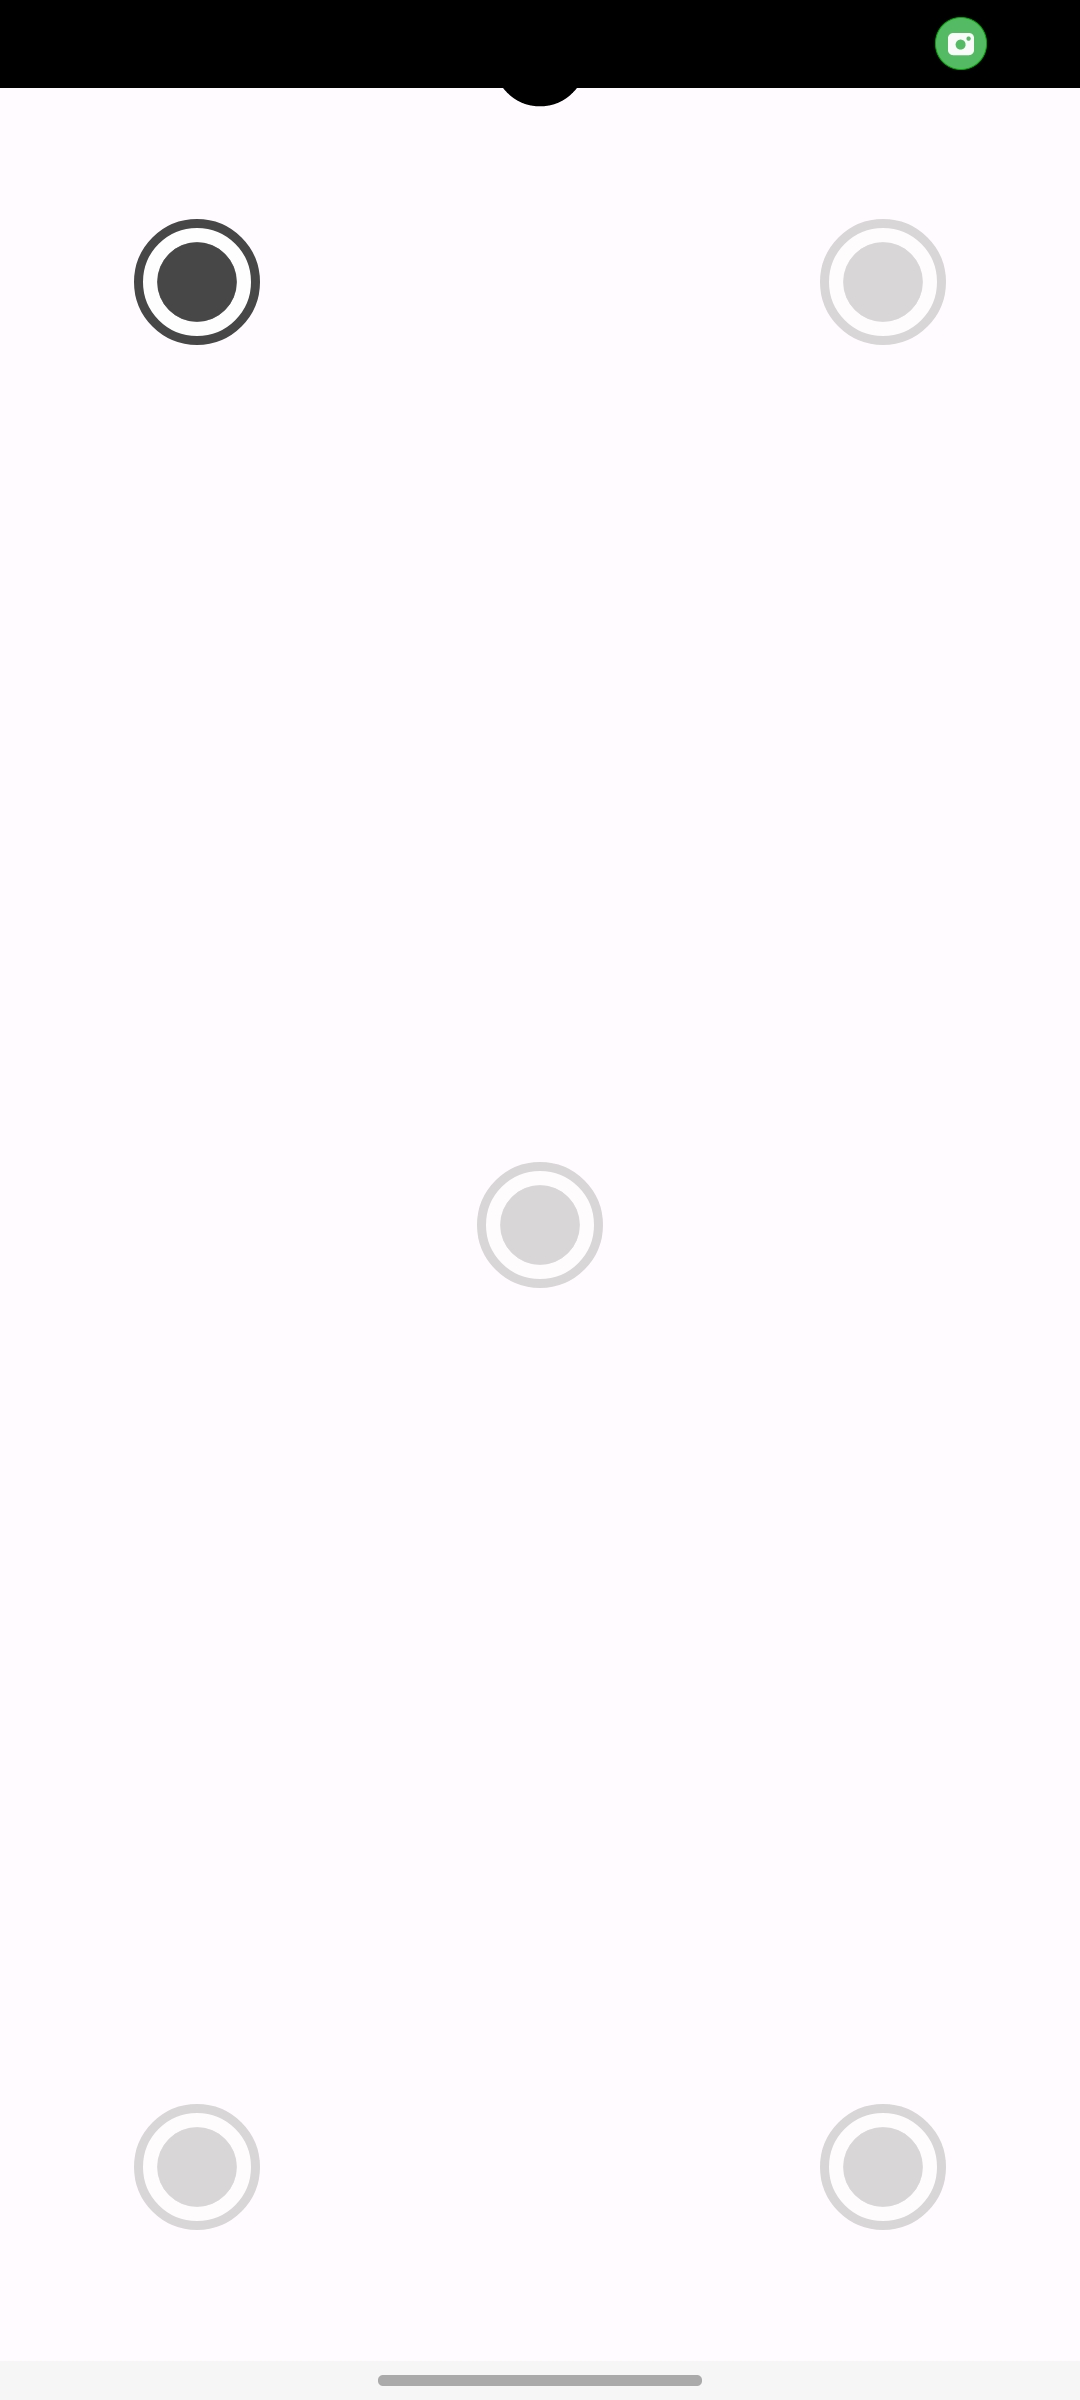
\includegraphics[scale=0.12]{ProgettoAndroid/Calibration/Images/CameraApp_Screen_calibration.jpg}
    \caption{Schermata Calibration}
    \label{fig:calibration}
\end{figure}

\section{Game}
\label{sec:game}
Nella fase di progettazione del gioco è stato deciso di implementare un gioco a quiz, in cui l'utente muovendo gli occhi avrebbe selezionato la risposta desiderata per la domanda sottoposta.

A tal proposito si è deciso di far riferimento al servizio OpentDB\cite{opentdb} (\textit{Open Trivia DB}) da cui tramite richieste $HTTP$ vengono acquisite 10 domande per iterazione in formato $JSON$. Successivamente vengono estratte solo le domande con quattro risposte possibili e mostrate a video i quesiti in modo sequenziale.

Il gioco in background abilita la fotocamera frontale e in tempo reale inizia il tracciamento degli occhi. Quando il tracciamento ha successo a video viene mostrato un cerchio rosso che rappresenta la posizione degli occhi. Muovendo gli occhi, e quindi il cerchio, su una risposta la si conferma. Se la risposta data è corretta il gioco mostrerà un'altra domanda fino a quando l'utente non sceglie di terminare il gioco.

\begin{figure}[htbp]
    \centering
    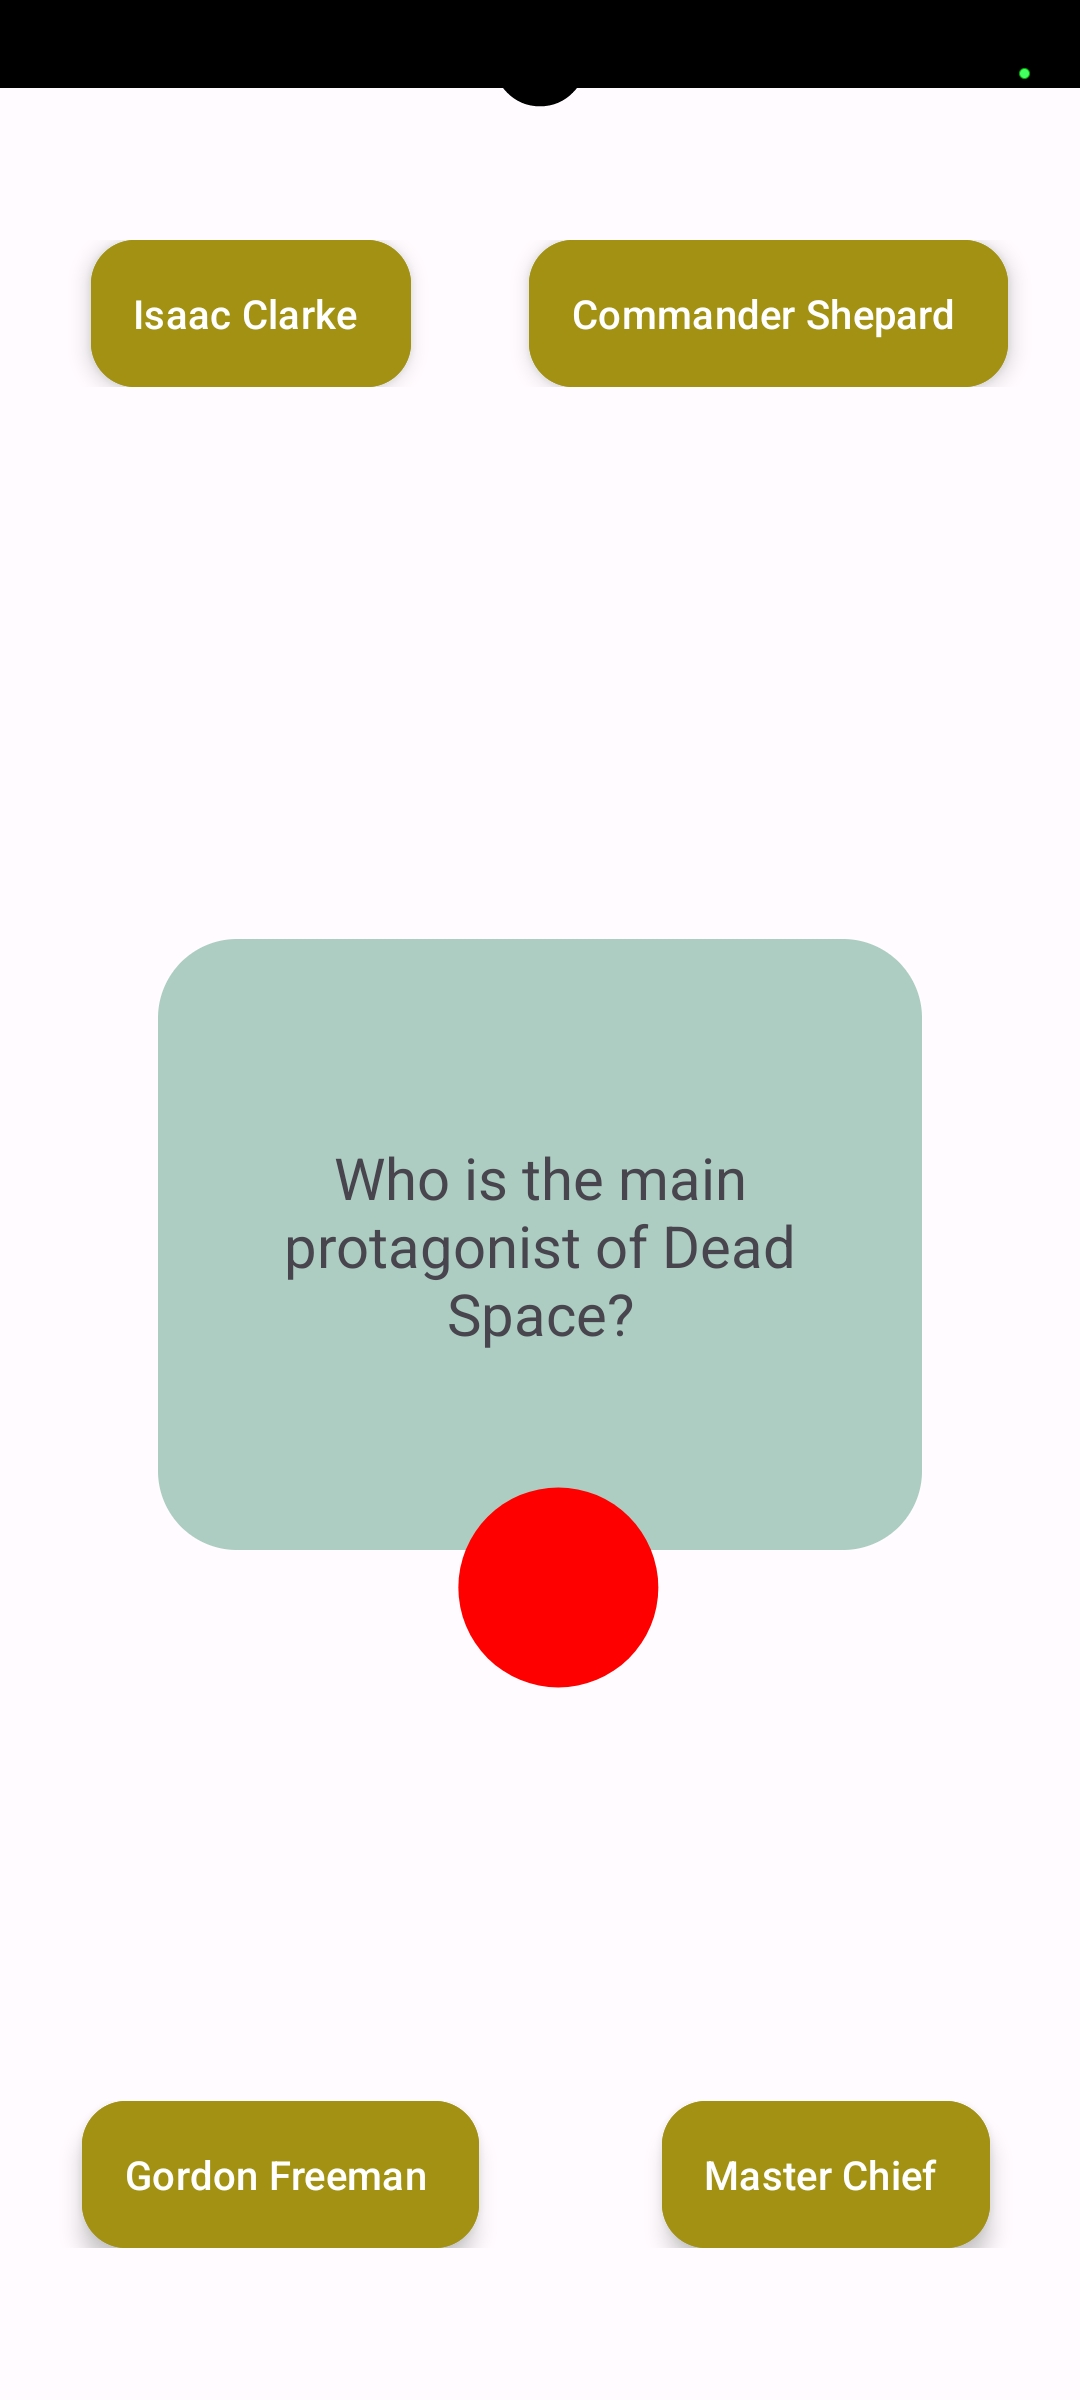
\includegraphics[scale=0.14]{ProgettoAndroid/Game/Images/CameraApp_Screen_quiz.jpg}
    \caption{Schermata Game}
    \label{fig:game}
\end{figure}

\section{Prestazioni}
\label{sec:prestazioni}
%\begin{figure}[htbp]
%    \centering
%    \subfigure[Static home]{
%    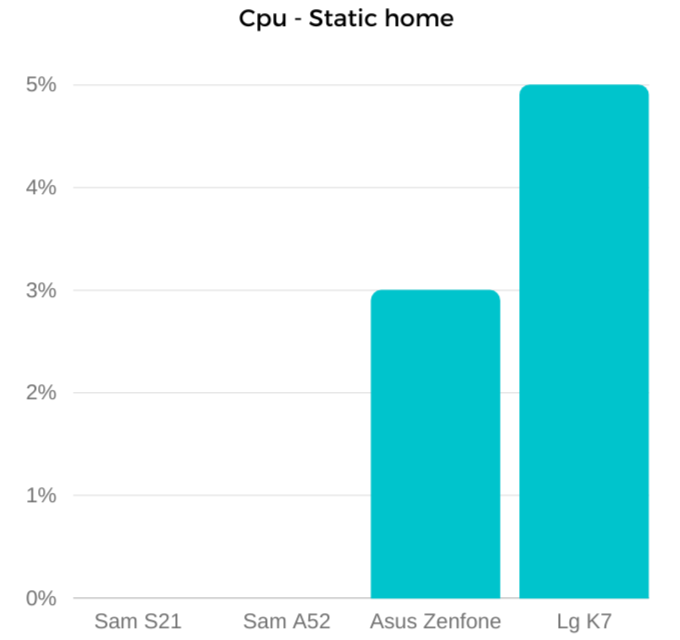
\includegraphics[scale=0.2]{ProgettoAndroid/Prestazioni/Images/Cpu-Static_home.png}
%    \label{fig:cpu_static_home}
%    }
    
%    \subfigure[Preview nerd]{
%    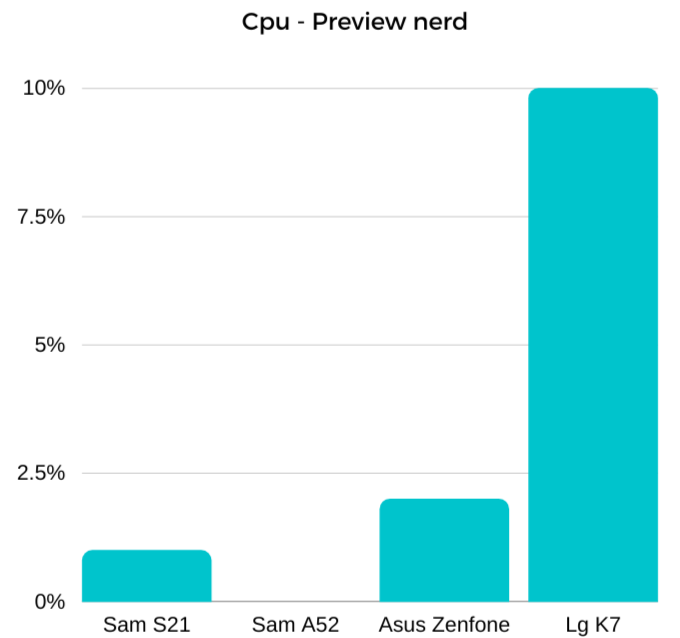
\includegraphics[scale=0.2]{ProgettoAndroid/Prestazioni/Images/Cpu-Preview_nerd.png}
%    \label{fig:cpu_preview_nerd}
%    }
    
%    \subfigure[Analysis nerd]{
%    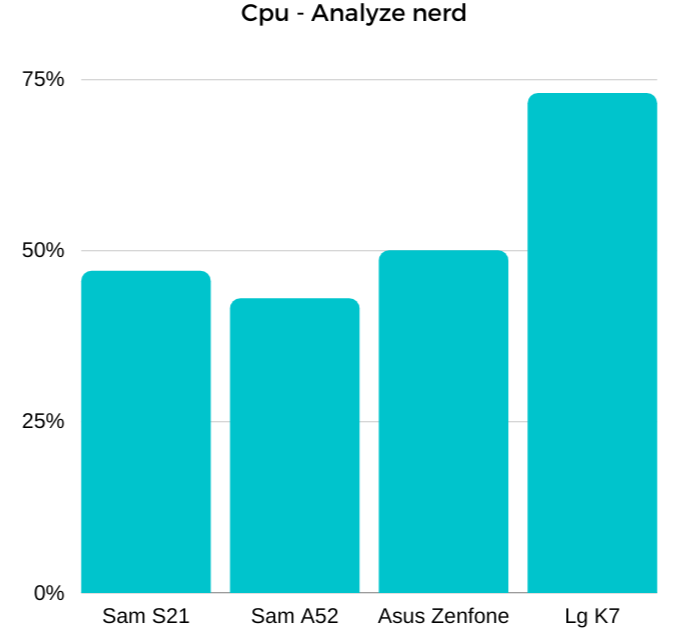
\includegraphics[scale=0.2]{ProgettoAndroid/Prestazioni/Images/Cpu-Analyze_nerd.png}
%    \label{fig:cpu_analysis_nerd}
%    }
    
%    \subfigure[Pupil nerd]{
%    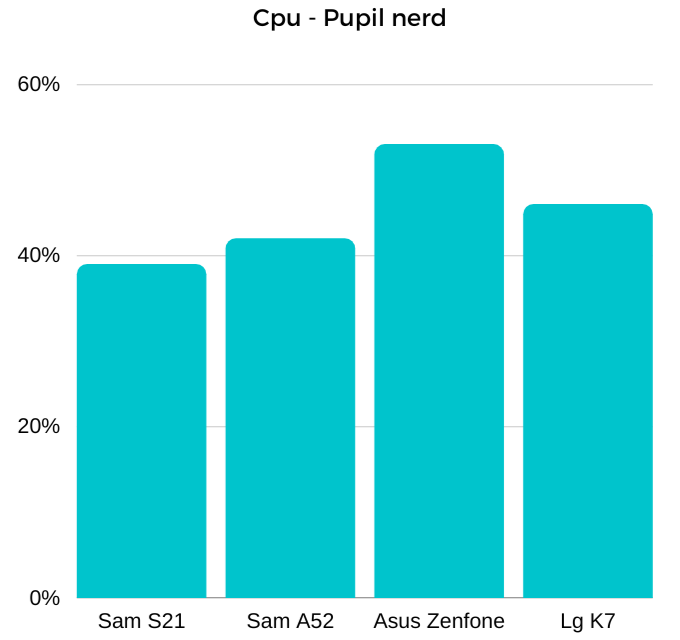
\includegraphics[scale=0.2]{ProgettoAndroid/Prestazioni/Images/Cpu-Pupil_nerd.png}
%    \label{fig:cpu_pupil_nerd}
%    }
    
%    \subfigure[Game]{
%    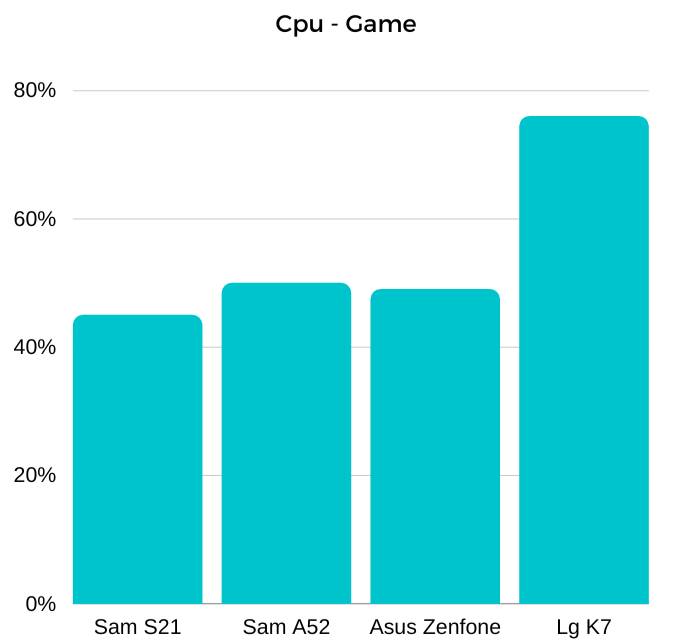
\includegraphics[scale=0.2]{ProgettoAndroid/Prestazioni/Images/Cpu-Game.png}
%    \label{fig:cpu_game}
%    }
    
%    \caption{CPU usage}
%    \label{fig:cpu_usage}
%\end{figure}
Di seguito vengono mostrati alcuni dati (l'utilizzo della CPU e della memoria) riguardanti le prestazioni lato Android utilizzando 4 differenti dispositivi.
\begin{figure}[htbp]
    \centering
    
    \subfigure[Static home]{
        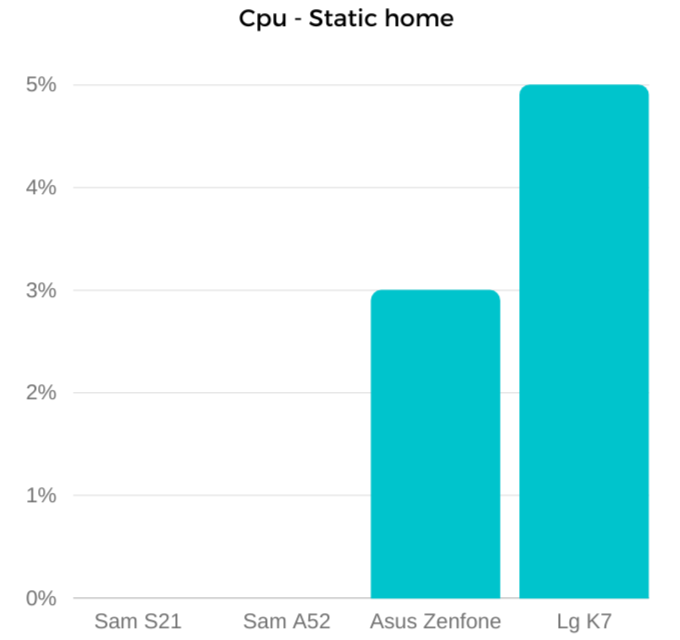
\includegraphics[scale=0.2]{ProgettoAndroid/Prestazioni/Images/Cpu-Static_home.png}
        \label{fig:cpu_static_home}
	}
    
    \subfigure[Preview nerd]{
        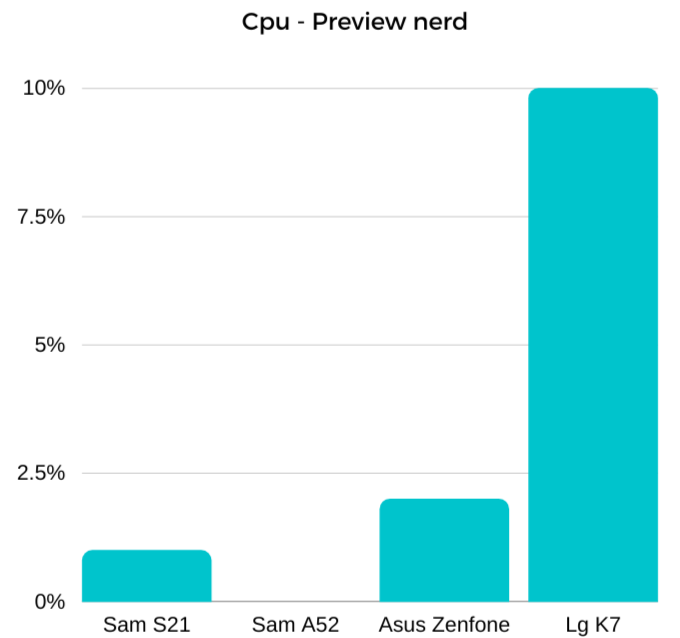
\includegraphics[scale=0.2]{ProgettoAndroid/Prestazioni/Images/Cpu-Preview_nerd.png}
        \label{fig:cpu_preview_nerd}
    }
    
    \subfigure[Analyze nerd]{
        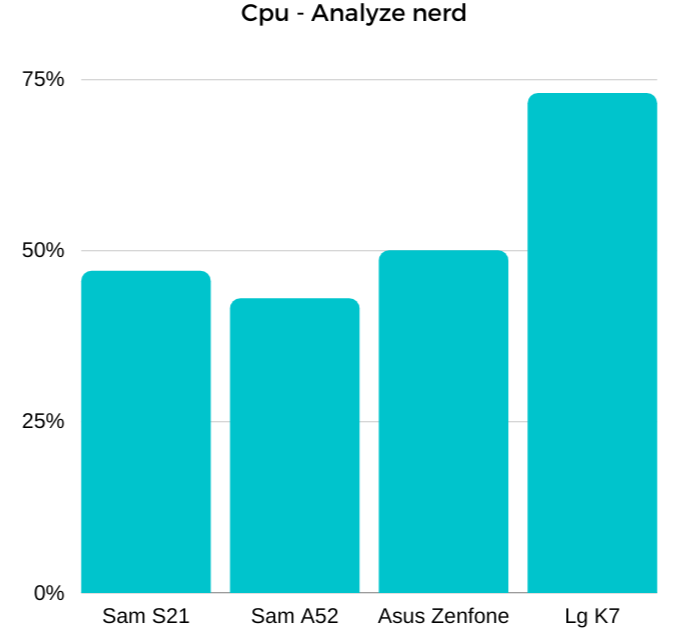
\includegraphics[scale=0.2]{ProgettoAndroid/Prestazioni/Images/Cpu-Analyze_nerd.png}
        \label{fig:cpu_analysis_nerd}
    }
    
    \subfigure[Pupil nerd]{
        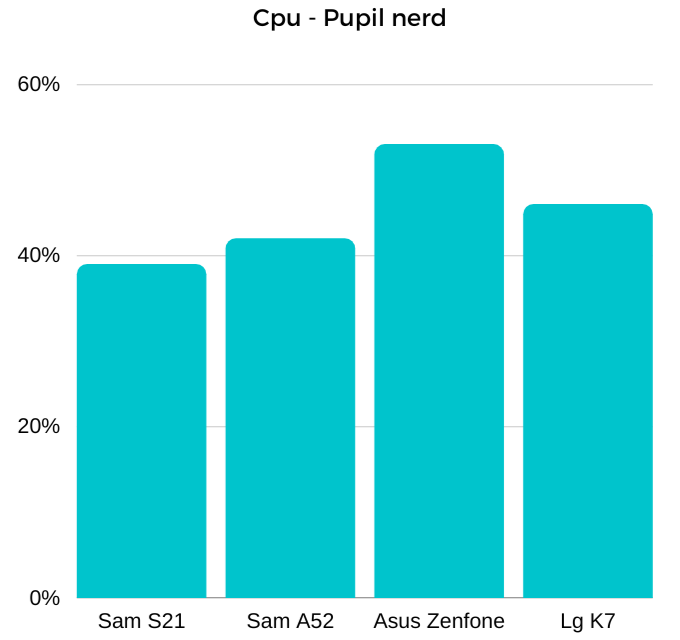
\includegraphics[scale=0.2]{ProgettoAndroid/Prestazioni/Images/Cpu-Pupil_nerd.png}
        \label{fig:cpu_pupil_nerd}
    }
    
    \subfigure[Game]{
        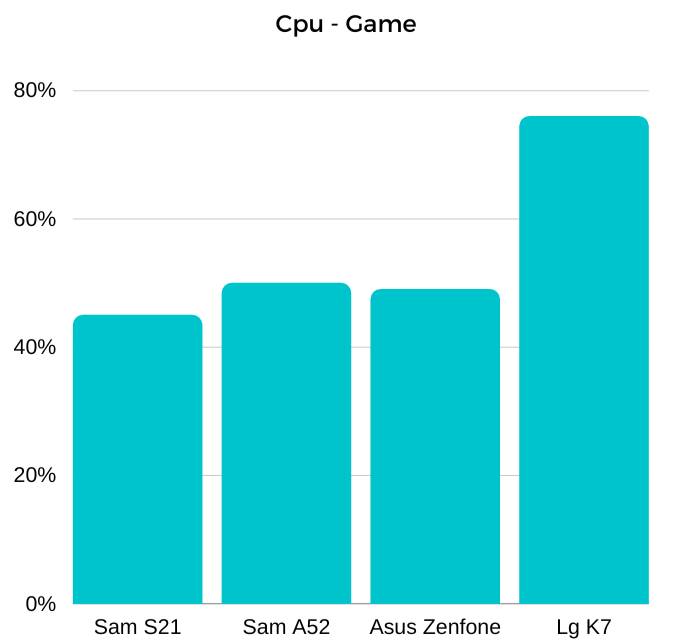
\includegraphics[scale=0.2]{ProgettoAndroid/Prestazioni/Images/Cpu-Game.png}
        \label{fig:cpu_game}
    }
    
    \caption{CPU usage}
    \label{fig:cpu_usage}
\end{figure}

\begin{figure}[htbp]
    \centering
    
    \subfigure[Static home]{
    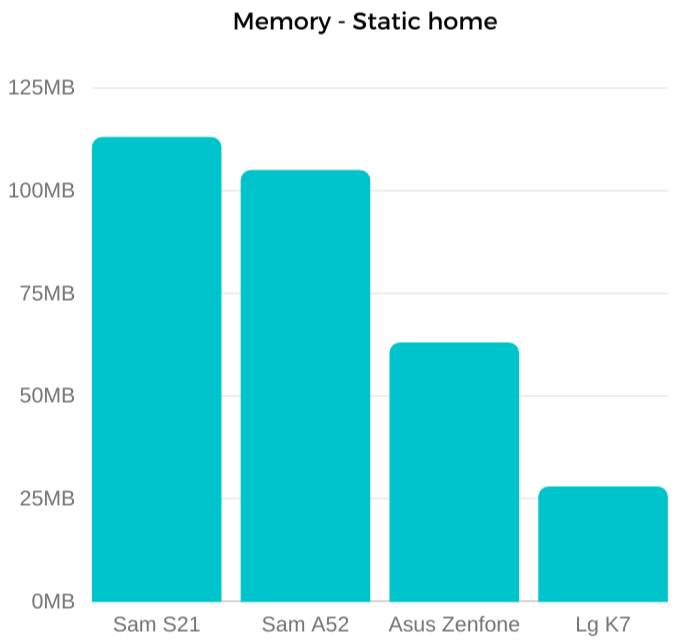
\includegraphics[scale=0.2]{ProgettoAndroid/Prestazioni/Images/Memory-Static_home.png}
    \label{fig:memory_static_home}
    }
    
    \subfigure[Preview nerd]{
    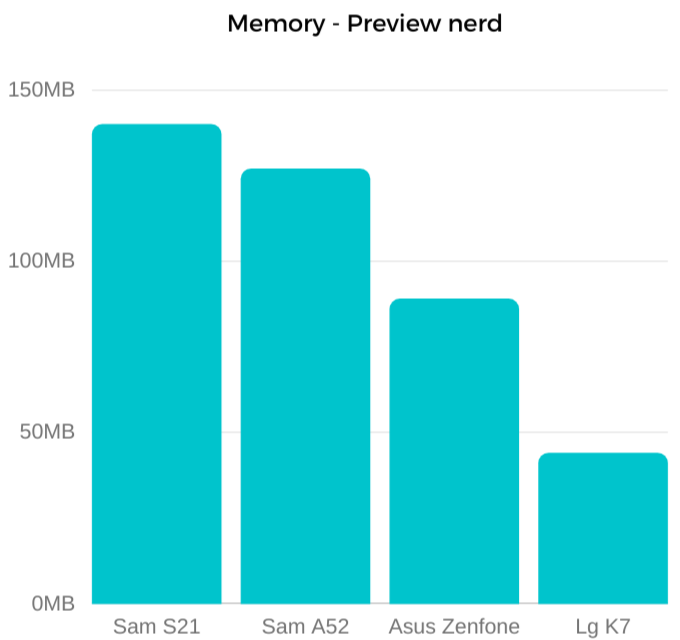
\includegraphics[scale=0.2]{ProgettoAndroid/Prestazioni/Images/Memory-Preview_nerd.png}
    \label{fig:memory_preview_nerd}
    }
    
    \subfigure[Analyze nerd]{
    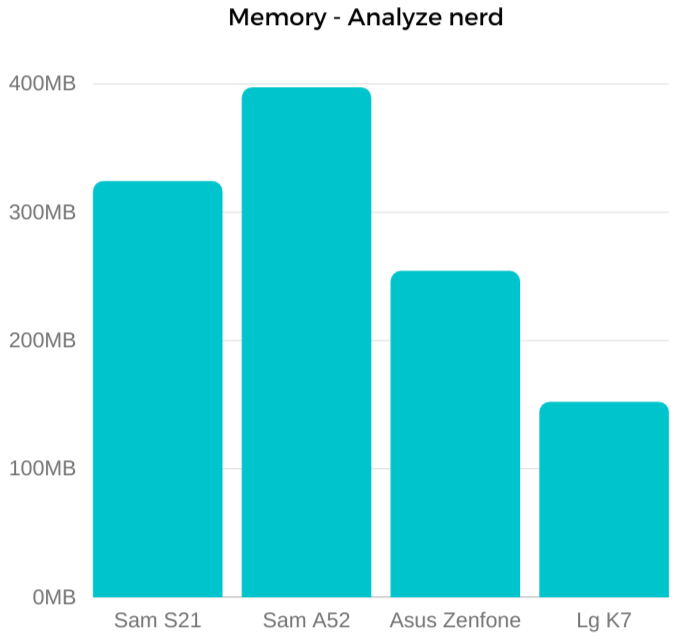
\includegraphics[scale=0.2]{ProgettoAndroid/Prestazioni/Images/Memory-Analyze_nerd.png}
    \label{fig:memory_analyze_nerd}
    }
    
    \subfigure[Pupil nerd]{
    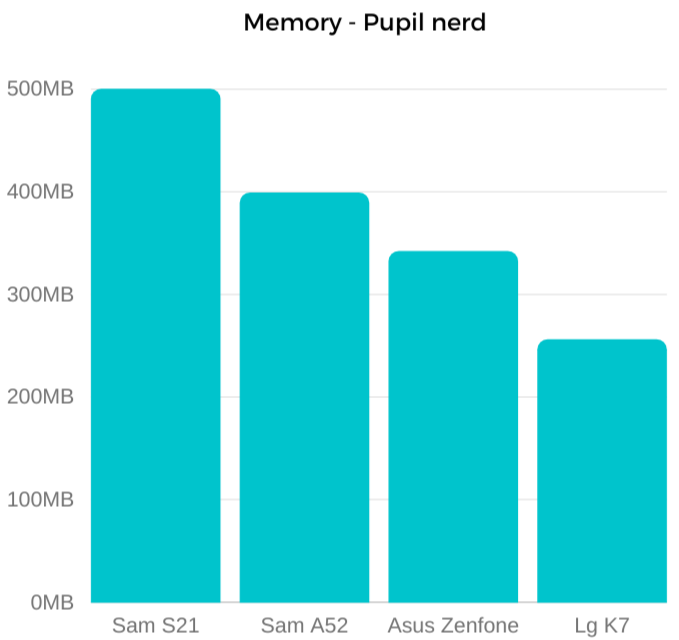
\includegraphics[scale=0.2]{ProgettoAndroid/Prestazioni/Images/Memory-Pupil_nerd.png}
    \label{fig:memory_pupil_nerd}
    }
    
    \subfigure[Game]{
    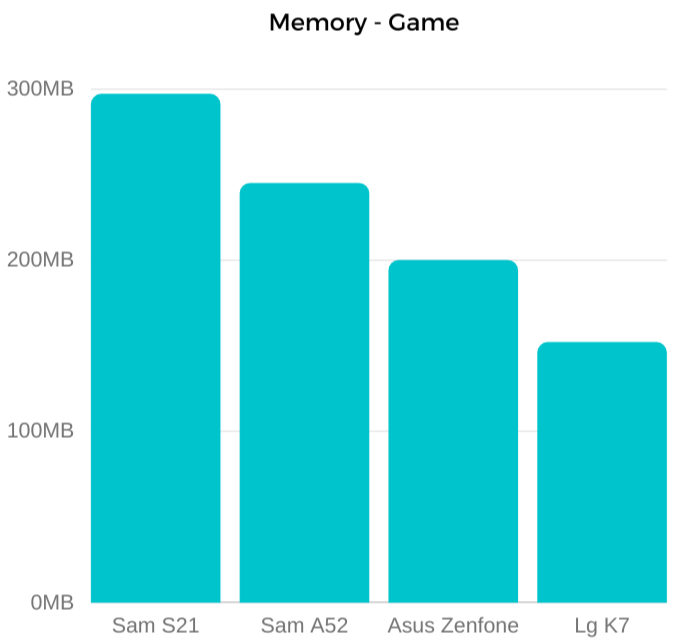
\includegraphics[scale=0.2]{ProgettoAndroid/Prestazioni/Images/Memory-Game.png}
    \label{fig:memory_game}
    }
    
    \caption{Memory usage}
    \label{fig:memory_usage}
\end{figure}